\documentclass{article}
%\usepackage[MeX]{polski}
%\usepackage[cp1250]{inputenc}
\usepackage{polski}
\usepackage[utf8]{inputenc}
\usepackage[pdftex]{hyperref}
\usepackage{makeidx}
\usepackage[tableposition=top]{caption}
\usepackage{algorithmic}
\usepackage{enumerate}
\usepackage{graphicx}
\usepackage{multirow}
\usepackage{amsmath} %pakiet matematyczny
\usepackage{amssymb} %pakiet dodatkowych symboli
\usepackage[table]{xcolor}
\usepackage{booktabs}
\usepackage{sidecap}
\usepackage{wrapfig}
\usepackage{caption}
\usepackage{subcaption}

\begin{document}





    \begin{table}
        \centering
        \caption{Multiprogram sets}
        \label{multiprogram}
        \begin{tabular}{c|c|c|c|c|c|c|c|c|}
            \cline{2-9}
             & \multicolumn{8}{|c|}{Sets}\\
            \cline{2-9}
             & 1 & 2 & 3 & 4 & 5 & 6 & 7 & 8\\
            \hline
            \multicolumn{1}{|c|}{astar} & & * &  & * &  &  & * &\\
            \hline
        \end{tabular}
    \end{table}
		
		
		
\begin{table}
\begin{center}
			\begin{tabular}{c|c|c|c|c|c|}
			\cline{2-6}
			\multirow{3}{*}{No. of visual words} & \multicolumn{5}{|c|}{Dataset} \\ \cline{2-6}
			  & 2 & 3 & 4 & 5 & 6 \\ \hline
			  & 7 & 7 & 7 & 7 & 7 \\ \hline
			
\end{tabular}
\caption{9 (Tabela 15) }
\end{center}
\end{table}













\begin{table}
\begin{center}
\rowcolors{1}{red}{green}
\begin{tabular}{ccc}
xxx & xxx & 333 \\
xxx & xzx & fdf \\
yyy & zzz & gdf \\
yyy & zzz & dgd \\
\end{tabular}
\caption{jedna kolorowa}

\end{center}
\end{table}

\begin{table}
\begin{center}
\begin{tabular}{c|c|c}
\hline
\hline 
$x_{1}$ & $x_{2}$ & ($x_{1}$AND$x_{2}$)  \\ \hline
1 & 1 & 1 \\ 
1 & 0 & 0 \\
0 & 1 & 0 \\
0 & 0 & 0 \\
\hline \hline
\end{tabular}
\caption{2 Tabela 11 }
\end{center}
\end{table}

\begin{table}
\begin{center}
\begin{tabular}{|r|l|}
\hline
7C0 & hexadecimal \\
3700 & octal \\ \cline{2-2}
11111000000 & binary \\ 
\hline
\hline 
1984 & decimal \\ \hline
\end{tabular}
\caption{Tabela 3 bez numeru}
\end{center}
\end{table}

\begin{figure}%
\caption{A picture of a R2D2}%
\centering
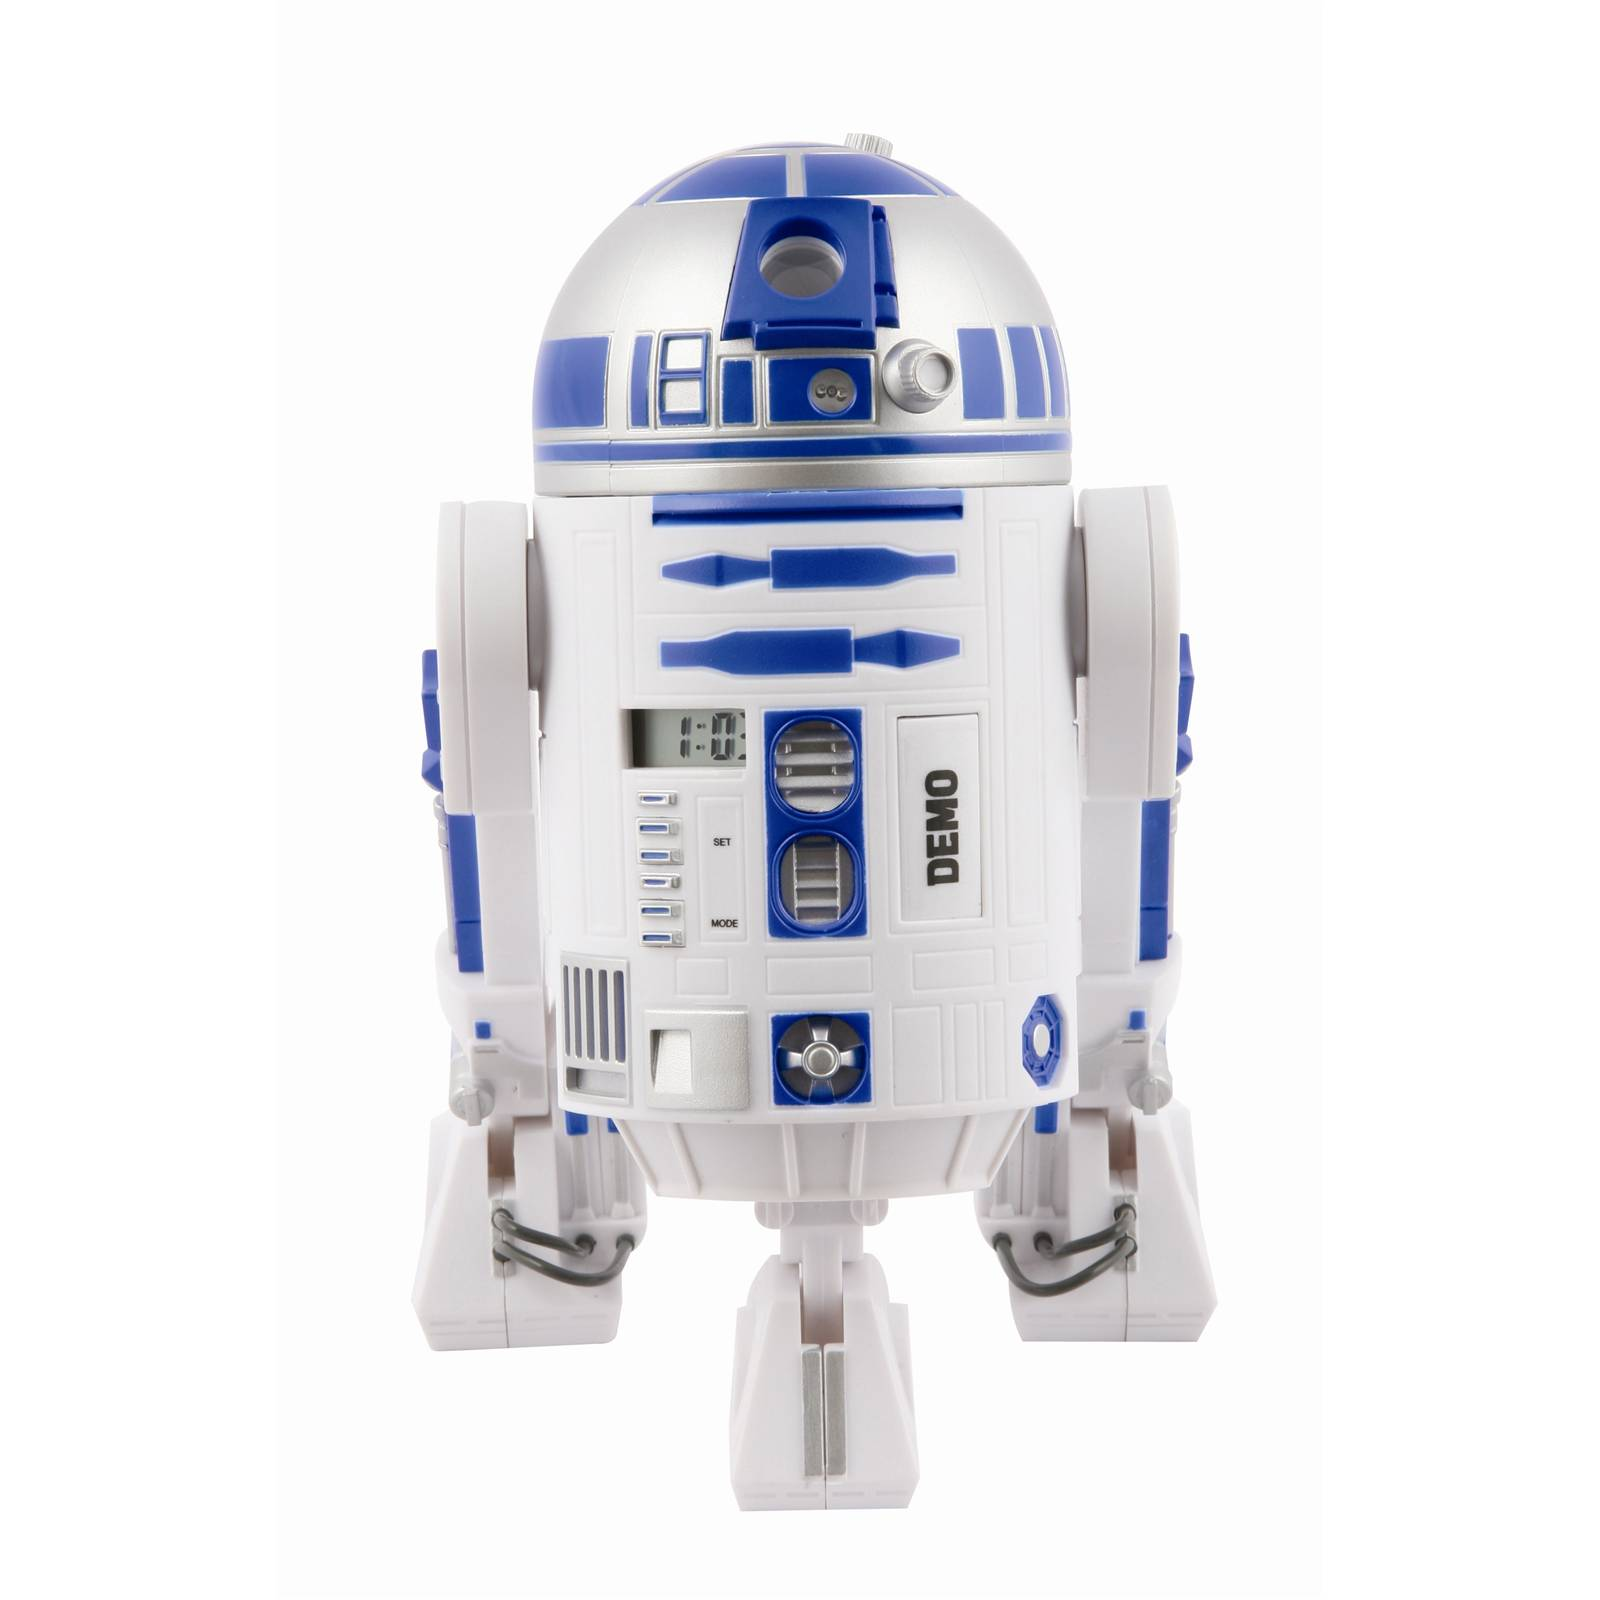
\includegraphics[width=\columnwidth]{R2D2.jpg}%
\end{figure}

\end{document}